% !TEX root = ../asfpp-user-manual.tex

\section{Using \asf}
\label{chap:using-asfpp}
This section describes how to succesfully perform simulations of cyber-physical attacks. Before running simulations, you have to build \asf succesfully (see section 1).

\subsection{Run your first attack}

\asf provides a set of ready-to-use simulation scenarios. We will use \texttt{chimneys-3smokes}:
%
\begin{lstlisting}[language={terminal}]
@~/asfpp $@ cd Simulations/chimneys-3smokes
\end{lstlisting}


\paragraph{Folder}
The folder \texttt{chimneys-3smokes} contains the following files and folders:
%
\begin{lstlisting}[language={terminal}]
@~/asfpp/Simulations/chimneys-3smokes@ ls
@attacks  chimneys-3smokes.pdf  omnetpp.ini  results  run.sh  scripts@
\end{lstlisting}
%
Files:
%
\begin{itemize}
\item \texttt{chimneys-3smokes.pdf} shows the simulation environment;
\item \texttt{omnetpp.ini} is the \texttt{ini} configuration file;
\item \texttt{run.sh} is a useful script that automatize the simulation process and the subsequent calculations.
\end{itemize}

Folders:
\begin{itemize}
\item \texttt{attacks} contains the attacks to permorm, it is provided with a set of redy-to-use attacks (\texttt{xml} with related \texttt{adl} files);
\item \texttt{scripts} contains the scripts used to perform the calculations to produce the values in which we are interested.
\item \texttt{results} contains the simulative results, it is provided with a set of already-executed simulations's results. 
\end{itemize}



\paragraph{Scenario}
Figure~\ref{fig:chimney-scenario} shows the referred scenario. 
%
\begin{figure}
\centering
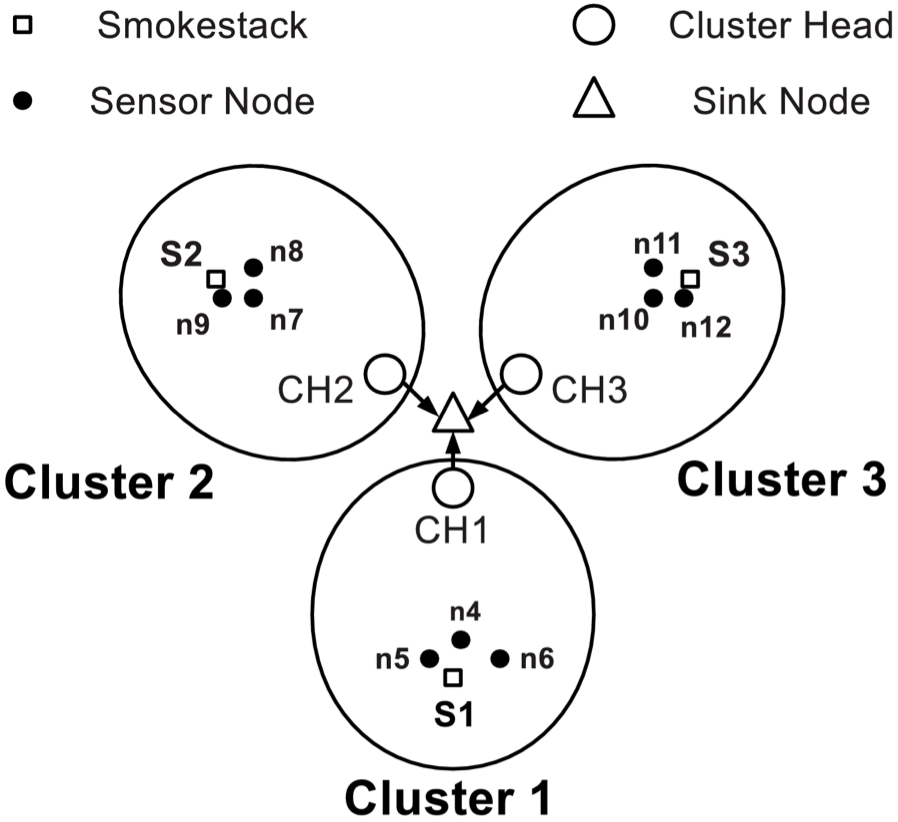
\includegraphics[width=.55\textwidth]{images/raster/scenario}
\caption{Chimney scenario}
\label{fig:chimney-scenario}
\end{figure} 
%
It consists of an industrial area in which three independent plants release pollutant into the air, through smokestack S1, S2 and S2 respectively. In the field there is also a WSN. It monitors pollution levels and detects any plants's abnormal behavior.

The WSN is composed by one sink and three clusters. Each cluster is associated with one smokestack and consists of one \emph{cluster head} and three \emph{sensor nodes}.

Each sensor node periodically senses the pollution in its own cluster and sends reports to its own cluster head. Periodically, each cluster head computes the average pollution level according to the received reports and delivers it to the sink node. Finally, the sink node checks whether any report exceeds a given threshold.

\paragraph{Configurations}
You can see all the possible configurations by following command: \footnote{If you have not exported the environment variable \texttt{~/asfpp/bin} as explained in the section~\ref{sec:asfpp-install}, you have to specify the entire relative path \texttt{../../bin/Castalia}.}
%
\begin{lstlisting}[language={terminal}]
@~/asfpp/Simulations/chimneys-3smokes $@ Castalia 
@
List of available input files and configurations:

* omnetpp.ini
	General
	misread
	misplace
	injection@
\end{lstlisting}

There are 4 different configurations. \texttt{General} is the Castalia's standard configuration, i.e. a configuration without cyber-physical attacks. \texttt{misread}, \texttt{misplace} and \texttt{injection} refer different attacks.

To automate the plotting of simulations's results, it is provided a bash script \texttt{run.sh}.


\subsubsection{General (no attack)}
\label{subsec:no-attack}
The first run refers to the configuration \texttt{General}.  If you are interested in the correctness of data, you can reapeat the simulation for $N$ times, for example 5:
%
\begin{lstlisting}[language={terminal}]
@~/asfpp/Simulations/chimneys-3smokes$@ ./run.sh
@
List of available input files and configurations:

* omnetpp.ini
	General
	misread
	misplace
	injection

Using input file 'omnetpp.ini'
Enter the 'Config' to run:@ General
@Using configuration 'General'
Enter the number of repetitions:@ 5
\end{lstlisting}

The script \texttt{run.sh} moves all the simulative results into a new folder, for example \texttt{General-20151014-172931}. The name of the new folder is that of the configuration that was used to which it is appended a timestamp.

Figure~\ref{fig:no-attack} (stored into the folder \texttt{plot}) shows the results of the simulation just performed.
%
\begin{figure}
\centering
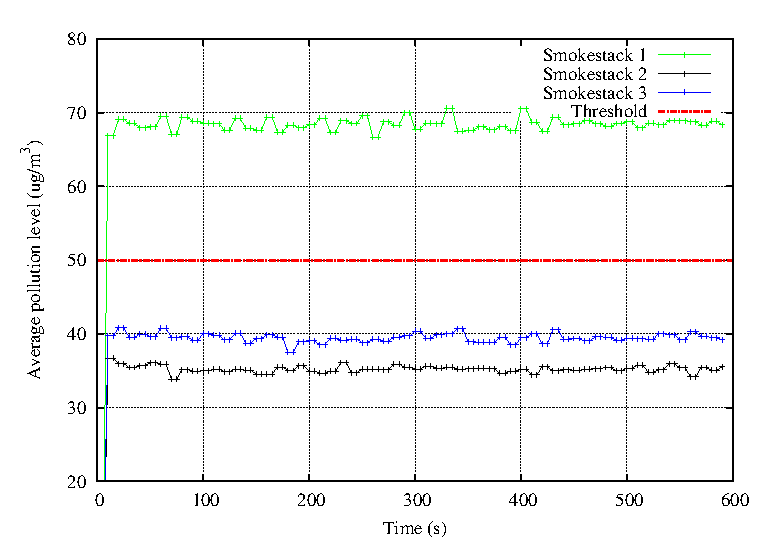
\includegraphics[width=.8\textwidth]{images/raster/general}
\caption{Results of configuration \texttt{General}}
\label{fig:no-attack}
\end{figure} 
%
The threshold (dashed red line) is fixed at 50 $\frac{\mu g}{m^3}$. The graph shows that emissions from S1 are exceeding the threshold.



\subsubsection{misread}
This is a \emph{physical} attack where sensor readings of 4, 5 and 6 tampered with the aim to lowering the value of their measurements.
%
\begin{lstlisting}[language={terminal}]
@~/asfpp/Simulations/chimneys-3smokes$@ ./run.sh
@
List of available input files and configurations:

* omnetpp.ini
	General
	misread
	misplace
	injection

Using input file 'omnetpp.ini'
Enter the 'Config' to run:@ misread
@Using configuration 'General'
Enter the number of repetitions:@ 5
\end{lstlisting}
%
Figure~\ref{fig:misread} shows the results of the simulation just performed.
%
\begin{figure}
\centering
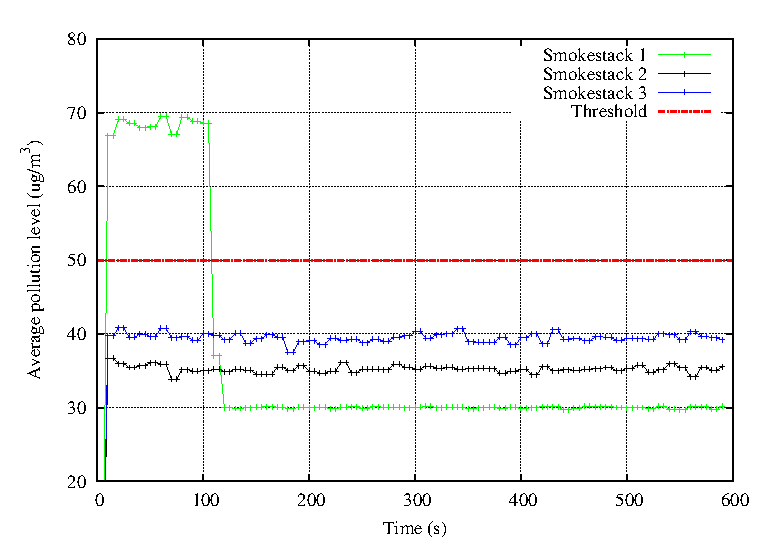
\includegraphics[width=.8\textwidth]{images/raster/misread}
\caption{Results of configuration \texttt{misread}}
\label{fig:misread}
\end{figure} 
%
By performing the attack \texttt{misread}, the emissions from S1 appear to be regular.


\subsubsection{misplace and injection}
You can run other ready-to-use attacks as explained above.



\subsection{Run your own attack}
\label{subsec:run-your-own-attack}
Before running your own attack, you must follow the following steps:
%
\begin{enumerate}
\item edit an \texttt{adl} file by using any text editor;
\item interpret the \texttt{adl} file by using the Attack Description Interpreter (ADI);
\item edit the file \texttt{omnetpp.ini} to include a configuration that refers the new attack.
\end{enumerate}


\paragraph{Write your own \texttt{adl} file}
To write your own attack you must know the Attack Description Language (ADL), see section \ref{sec:adl}. You can write a new attack by editing editing a new \texttt{adl} file. For example, we can create the file \texttt{destroy.asl} that contains the description of an attack that destroys nodes 4, 5 and 6.
%
\begin{lstlisting}[language={adl}]
# destroy attack
destroy(4, 100)
destroy(5, 100)
destroy(6, 100)
\end{lstlisting}

\paragraph{Interpret the \texttt{adl} file}
After creating the file that contains the description of the attack, you have to intepret it by using the ADI. The general sintax to invoke the ADI is the following:
%
\begin{lstlisting}[language={terminal}]
python path/interpreter.py -i <file.adl> -o <file.xml>
\end{lstlisting}
%
The input file is mandatory. You can specify the name of the \texttt{xml} file, that is the output of the ADI. If the file \texttt{destroy.adl} is stored in \texttt{~/asfpp/Simulations/chimneys-3smokes/attacks}, to interpret it type:
%
\begin{lstlisting}[language={terminal}]
@~/asfpp/Simulations/chimneys-3smokes/attacks$@ python ../../../interpreter/interpreter/interpreter.py -i destroy.adl
@Using default output filename 'destroy.xml'@
\end{lstlisting}
%
The output file is \texttt{destroy.xml}.


\paragraph{Edit the file \texttt{omnetpp.ini}}
The last step is to edit the configuration file \texttt{omnetpp.ini}. It is composed of several parts, each of which describes a particular configuration.
The firsts part is always referred to the configuration \texttt{General}, which is mandatory. After the configuration \texttt{General}, you can describe other configurations. 

To describe a new configuration that includes the file \texttt{destroy.xml}, you have to append to the configuration file the following lines:
%
\begin{lstlisting}[language={terminal}]
[Config destroy]
SN.configurationFile = "attacks/destroy.xml"
\end{lstlisting}
%
For a better understanding about the configuration file, see the user manuals of \omnet and Castalia. 

\paragraph{Run the simulation}
Finally you can run the simulation that includes the attack destroy.